\subsection{Properties of Relevant Isotopes and Fuel Salt}
\label{sec:fuelSaltProperties}
There are three isotopes we are chiefly concerned with, $^{135}Te$, $^{135}I$, and $^{135}Xe$.  Collectively, we shall refer to these isotopes as the \textit{poison isotopes} Some analyses, such as that in ORNL-TM-1070 ignore Tellerium.  The effects of $^{135m}Xe$ have also been investigated in ORNL-TM-3464 and by Eades.\cite{ORNLTM3464,Eades16}  

The poison species progress down the decay chain through nuclear decay. The $^{135}Te \rightarrow ^{135}I \rightarrow ^{135}Xe$ chain with a $^{135m}Xe$ branch is depicted in figure \ref{fig:XeDecay}. \begin{figure}[ht]
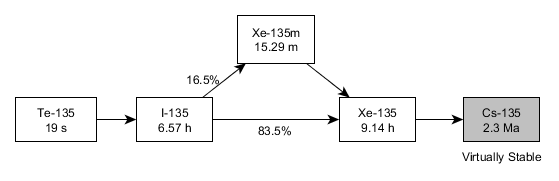
\includegraphics[width=\textwidth,height=\textheight,keepaspectratio]{XeDecay.png} 
\caption{Xe Decay Chain}
\label{fig:XeDecay}
\end{figure} Te-135 decays into I-135 through beta minus decay with a 19 s half-life. \cite[p. 56]{Baum2010}  Iodine then undergoes beta minus decay and transmutes into either Xe-135 or the meta-stable form, Xe-135m  6.57 h half-life. [ibid.] Any Xe-135m formed de-excites into Xe-135 through gamma emanation with a 15.3 m half-life. \cite[p. 298]{Eades16} Xe-135 finally transmutes into Cs-135 with a half-life of 9.14h.\cite[p. 56]{Baum2010} The Cs-135 is virtually stable with its 2.3 My half-life. [ibid]  All of these poison isotopes are both produced directly from fission, as the product of other nuclear reactions, and from radioactive decay.

The thermal neutron absorption cross section for xenon-135 is 2.6 Mb. \cite[p. 54-9]{Mughab12P1} The neutron absorption cross section for Xe-135 averaged over the MSRE neutron spectrum is 1.18 Mb\footnote{This claim is based on a personal communication between the authors of ORNL-4069 and B.E. Prince.  No details as to how this value was arrived at are given.}.\cite[p. 42]{ORNL4069} [ The xenon model in ORNL-4069 did not include any considerations of Xe-135m; however, the xenon model in ORNL-TM-3464 did. The ORNL-TM-3464 xenon model did not include any consideration for neutron absorption in Xe-135m since the cross-section was was unknown at the time. \cite[p. 3]{ORNLTM3464}  Since then, Eades, who reported the Xe-135m thermal neutron absorption cross-section is 10 Mb, has investigated its effect on MSRs.\cite{Eades16}

The thermophysical properties of molten salt influence the behavior of xenon in an MSR.  Yoder warns that the accuracy of heat transfer correlations in molten salt systems are limited by the accuracy of the thermophysical properties.\cite{Yoder2014} By extension, the accuracy of mass-transfer correlations, through heat/mass transfer analogies, are limited by the accuracy of thermophysical properties.  Some sources of thermophysical data are for use in modeling efforts are given by Cantor, Sohal, and Janz. \cite{ORNLTM2316,Sohal2010,Janz2013} In the work by Cantor, fuel salt F4 is closest in composition to enriched MSRE fuel salt as given in ORNL-TM-0728.  The uranium enrichment of fuel-salt F4 was not found. Nevertheless, given the 1.3\% difference in mass between U-235 and U-238 is about 1.3\%, the difference in thermophysical properties between enriched an unenriched fuel salt can be assumed to be negligible.  In addition to these data, Grimes, Blander, and Watson give information on solubility limits and Henry’s constants for xenon and other noble gases.\cite{Grimes1958, Blander1959, Watson1962} Note the temperature and pressure dependence of Henry’s constants and xenon solubility limits. 
